%%%%%%%%%%%%%%%%%%%%%%%%%%%%%%%%%%%%%%%%%%%%%%%%%%%%%%%%%%%%%%%%%%%%%%%%
\documentclass[12pt]{article}
\usepackage{amssymb}
\usepackage{amsmath,amssymb,CJK}
\usepackage{array}
\usepackage{graphicx}
\usepackage{subfigure}
\usepackage{listings}
\usepackage{epstopdf}

\openup 7pt\pagestyle{plain} \topmargin -40pt \textwidth
14.5cm\textheight 21.5cm
\parskip .09 truein
\baselineskip 4pt\lineskip 4pt \setcounter{page}{1}
\def\a{\alpha}\def\b{\beta}\def\d{\delta}\def\D{\Delta}\def\fs{\footnotesize}
\def\g{\gamma}
\def\G{\Gamma}\def\l{\lambda}\def\L{\Lambda}\def\o{\omiga}\def\p{\psi}
\def\se{\subseteq}\def\seq{\subseteq}\def\Si{\Sigma}\def\si{\sigma}\def\vp{\varphi}\def\es{\varepsilon}
\def\sc{\scriptstyle}\def\ssc{\scriptscriptstyle}\def\dis{\displaystyle}
\def\cl{\centerline}\def\ll{\leftline}\def\rl{\rightline}\def\nl{\newline}
\def\ol{\overline}\def\ul{\underline}\def\wt{\widetilde}\def\wh{\widehat}
\def\rar{\rightarrow}\def\Rar{\Rightarrow}\def\lar{\leftarrow}
\def\Lar{\Leftarrow}\def\Rla{\rightleftarrow}\def\bs{\backslash}
\def\ra{\rangle}\def\la{\langle}\def\hs{\hspace*}\def\rb{\raisebox}
\def\ni{\noindent}\def\hi{\hangindent}\def\ha{\hangafter}
\def\vs{\vspace*}
\def\hom#1{\mbox{\rm Hom($#1,#1$)}}
\def\thebeg{\vskip8pt\par\ni}
\def\theend{\vskip5pt\par}
\def\chabeg{\pagebreak\par}
\def\chaend{\vskip20pt\par}
\def\secbeg{\vskip15pt\par}
\def\secend{\vskip10pt\par}
\def\exebeg{\vskip10pt}
\def\exeend{\vskip6pt}
\def\undot#1{\mbox{$\mbox{#1}\hs{-1.5ex}_{_{\dis\centerdot}}\,\,$}}
\def\qed{\hfill\mbox{$\Box$}}
\def\C{\mathbb{C}}
\def\Q{\mathbb{Q}}
\def\ii{\mbox{\,{\bf i}\,}}
\def\jj{\mbox{\,{\bf j}\,}}
\def\AA{{\cal A}}
\def\BB{{\cal B}}
\def\DD{{\cal D}}
\def\EE{{\mbox{\bf 1}}}
\def\OO{{\mbox{\bf 0}}}
\def\kk{{\mbox{\bf k}}}
\def\R{\mathbb{R}}
\def\F{\mathbb{F}{\ssc\,}}
%\def\similar{\rb{-4pt}{\mbox{\,\~\,}}}
\def\similar{\backsim}
\def\Llra{\Longleftrightarrow}
\def\Lra{\Longrightarrow}
\def\Lla{\Longleftarrow}
\def\mat#1#2{\mbox{$\left(\begin{array}{#1}#2\end{array}\right)$}}
\def\det#1#2{\mbox{$\left|\begin{array}{#1}#2\end{array}\right|$}}
\def\eset{\emptyset}
\parindent=5ex
\setlength{\parindent}{0pt}
\setlength{\parskip}{1ex plus 0.5ex minus 0.2ex}
\newtheorem{Example}{\text{例}}

\begin{document}
\begin{CJK*}{UTF8}{gbsn}

\date{}
\title{行星的轨道和位置}
\author{李青林,5110309074\\郑辉煌,5110209289}
\maketitle

\section{实验任务1}
\subsection*{问题}
在求解方程$(5.24)$时,试用矩形法和simpson法来计算数值积分,并对所得的结果加以比较

\subsection*{解答}
矩形法:\\
\begin{lstlisting}[language = matlab]
function Q1_rectangle(h)
    ep=0.01672;  C1=4.455e15;  p=1.496e11;
    T1=100*24*3600;  f=C1*T1/p^2;
    theta=0;  F=0;

    i=2;
    while true
        theta=theta+h;
        F=F+h*(1-ep*cos((theta-h/2)))^-2;
        if F>f; break;end
        i=i+1;
    end

    t=theta-h;  r=p/(1-ep*cos(t));
    dtheta=C1/r^2;  v=r*dtheta;
    disp(h);disp(t);disp(v);
end

\end{lstlisting}

\begin{tabular}{|c|c|c|}
\hline
h & $\theta$ & v \\
\hline
0.1 & 1.6000 & 29794 \\
\hline
0.01 & 1.6800 & 29834 \\
\hline
0.001 & 1.6850 & 29836 \\
\hline
0.0001 & 1.6859 & 29837 \\
\hline
0.00001 & 1.6860 & 29837 \\
\hline
\end{tabular}

simpson法:\\
\begin{lstlisting}[language = matlab]
function Q1_simpson(h)
    ep=0.01672;  C1=4.455e15;  p=1.496e11;
    T1=100*24*3600;  f=C1*T1/p^2;  theta=0;
    F=0;  fun=@(x)(1-ep*cos(x))^-2;

    i=2;
    while  true
        theta=theta+h;
        F=F+h/6*(fun(theta-h)+4*fun(theta-h/2)+fun(theta));
        if F>f;break;end
        i=i+1;
    end

    t=theta-h;  r=p/(1-ep*cos(t));
    dtheta=C1/r^2;  v=r*dtheta;
    disp(h);disp(t);disp(v);
end

\end{lstlisting}

\begin{tabular}{|c|c|c|}
\hline
h&$\theta$&v\\
\hline
0.1&1.6000&29794\\
\hline
0.01&1.6800&29834\\
\hline
0.001&1.6850&29836\\
\hline
0.0001&1.6859&29837\\
\hline
0.00001&1.6860&29837\\
\hline
\end{tabular}

可以看出由于精度受步长限制,试用精度更高的simpson公式并不会使得计算量大幅减小\\

\section{实验任务2}
\subsection*{问题}
水星到太阳的最远距离为$0.6982\times10^{11}$m,此时水星绕太阳运行的线速度是$3.886\times10^4$m/s,试求:
\begin{enumerate}
\item
水星到太阳的最近距离

\item
水星绕太阳运行的周期

\item
画出水星绕太阳旋转的轨道曲线

\item
求从远日点开始的第$50$天(地球天)结束时水星的位置

\end{enumerate}

\subsection*{解答}
\begin{enumerate}
\item
已知$$r_0=0.6982\times10^{11}, v_0=3.886\times10^4$$
由行星轨迹方程$$r=\frac{p}{1-e\cos\theta}$$
得$\theta=\pi$时,$r$最小,为近日点\\
$$r_m=\frac{p}{1+e}$$
可知$$C_1=2.7132\times10^{15}, p=\frac{C_1^2}{MG}=5.5472\times10^{10}$$
$$e=1-\dfrac{p}{r_0}=0.2055$$
则最近距离为$$r_m=4.6016\times10^{10}(\mathrm{m})$$

\item
设周期为$T$,由开普勒第二定律$$\int_0^T\dfrac{1}{2}r^2\dfrac{\mathrm{d}\theta}{\mathrm{d}t}\mathrm{d}\theta=\dfrac{1}{2}C_1T$$
上式左端为行星轨迹椭圆所围的面积,记为$S$
$$S=\pi ab=\frac{\pi p^2}{(1-e^2)^{\frac{3}{2}}}$$
代入,解得
$$T=\frac{2\pi p^2}{C_1(1-e^2)^\frac{3}{2}}=7.6025\times10^6(\mathrm{s})=87.991(\mathrm{d})$$

试用runge-kutta法:
\begin{lstlisting}[language=matlab]
function Q2_4(h)
    function dy=build(t,y)
        C1=2.7132e+015;MG=1.3271e+020;
        dy=[C1^2/y(2)^3-MG/y(2)^2;y(1);C1/y(2)^2];
    end
[t,y]=ode45(@build,0:h:100*24*3600,[0,0.6982e11,0]);
n=find(y(:,3)<2*pi,1,'last');
T=t(n);
r=y(round(n/2),2);
disp(T/24/3600);disp(r);
polar(y(:,3),y(:,2));
end
\end{lstlisting}
得出$T=87.8472(\mathrm{d}),r_m=4.6002\times10^{10}(\mathrm{m})$,与理论计算相符
\item
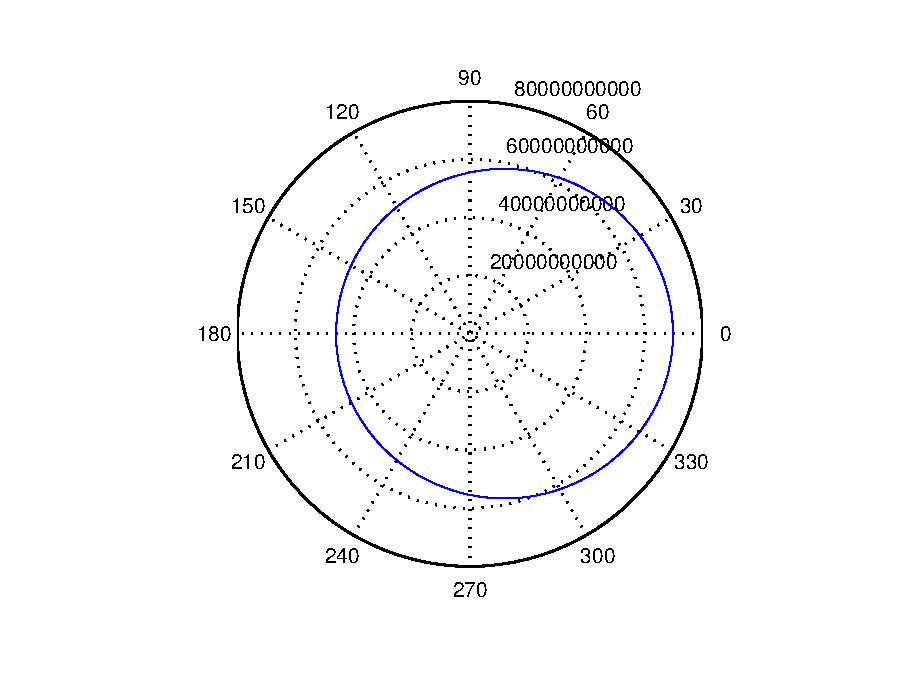
\includegraphics[scale=1]{Q2_3.eps}

\item
由开普勒第二定律$$\int_\theta^{\theta+\Delta\theta}r^2\mathrm{d}\theta=C_1\Delta t$$
可得$$\int_0^\theta\frac{p^2}{C_1(1-e\cos\theta)}\mathrm{d}\theta=t$$
解方程$$F(\theta)=\frac{C_1T_1}{p^2}$$
其中$$F(\theta)=\int_0^\theta\frac{1}{(1-e\cos\phi)}\mathrm{d}\phi$$
\newpage
simpson法:
\begin{lstlisting}[language=matlab]
function Q2_4_simpson(h)
ep=0.2055;C1=2.7132e15;p=5.5472e10;
T1=50*24*3600;f=C1*T1/p^2;theta=0;
F=0;fun=@(x)(1-ep*cos(x))^-2;

i=2;
while true
    theta=theta+h;
    F=F+h/6*(fun(theta-h)+4*fun(theta-h/2)+fun(theta));
    if F>f;break;end
    i=i+1;
end

t=theta-h;r=p/(1-ep*cos(t));
dtheta=C1/r^2;v=r*dtheta;
disp(r);disp(t);disp(v);
end

\end{lstlisting}

\begin{tabular}{|c|c|c|c|}
\hline
h&r($\times10^{10}$) & $\theta$ & v($\times10^4$) \\
\hline
 0.1&4.7239&3.7000&5.7436\\
\hline
0.01&4.7665&3.7900&5.6922\\
\hline
0.001&4.7665&3.7900&5.6922\\
\hline
0.0001&4.7668&3.7906&5.6919\\
\hline
0.00001&4.7668&3.7906&5.6919 \\
\hline
\end{tabular}

得$50$天后水星处于$r=4.7668\times10^{10}\mathrm{(m)}$,$\theta=3.7906$处,$v=5.6919\mathrm{(m/s)}$

runge-kutta法:
\begin{lstlisting}[language=matlab]
function Q2_4
    function dy=build(t,y)
        C1=2.7132e+015;MG=1.3271e+020;
        dy=[C1^2/y(2)^3-MG/y(2)^2;y(1);C1/y(2)^2];
    end
[t,y]=ode45(@build,[0 50*24*3600],[0,0.6982e11,0]);
disp(y(length(y),2));disp(y(length(y),3));
end
\end{lstlisting}
求得$  r=4.7667\times10^{10}\mathrm{(m)},\theta=3.7909$\\
%实验得知,要得到相同的精度,simpson法比runge-kutta法慢

\end{enumerate}

\section{实验任务3}
\subsection*{问题}
利用开普勒三定律,也可以推导出万有引力定律,试完成这个推导
\subsection*{解答}
\begin{enumerate}
\item
开普勒第一定律:行星的轨道是椭圆,太阳位于椭圆的一个焦点上。\\
椭圆轨道极坐标方程为:
$$\frac{ep}{1-ecos\theta}$$
以位矢的观点看:
$$\textbf{r} = r \textbf{i}$$
\textbf{i}为径向单位向量,另外设\textbf{j}为切向单位向量,则
$$\frac{d\textbf{i}}{dt} = \frac{d\theta}{dt}\textbf{j}$$
$$\frac{d\textbf{j}}{dt} = -\frac{d\theta}{dt}\textbf{i}$$
从而对速度矢量\textbf{v}有:
$$\textbf{v} = \frac{d\textbf{r}}{dt} = \frac{dr}{dt}\textbf{i} + r \frac{d\textbf{i}}{dt} = \frac{dr}{dt}\textbf{i} + r\frac{d\theta}{dt}\textbf{j}$$
记再得到加速度的表达式
\begin{align*}
\textbf{a} &= \frac{d\textbf{v}}{dt}\\
           &= \frac{d\dot{r}i}{dt} + \frac{dr\dot{\theta}j}{dt}\\
           &= (\ddot{r}i + \dot{r}\frac{di}{dt}) + (\dot{r}\dot{\theta}j + r\ddot{\theta}j + r\dot{\theta}\frac{dj}{dt})\\
           &= (\ddot{r}i + \dot{r}\dot{\theta}j) + (\dot{r}\dot{\theta}j + r\ddot{\theta}j - r\dot{\theta}^{2}i)\\
           &= (\ddot{r} - r\dot{\theta}^{2})i + (r\ddot{\theta} + 2\dot{r}\dot{\theta})j
\end{align*}
故径向和横向加速度分别为:
$$a_{r} = \ddot{r} - r\dot{\theta}^{2}$$
$$a_{\theta} = r\ddot{\theta} + 2\dot{r}\dot{\theta}$$
那么首先
$$a_{\theta} = r\ddot{\theta} + 2\dot{r}\dot{\theta} = \frac{1}{r}(2r\dot{r}\dot{\theta} + r^{2}\ddot{\theta}) = \frac{1}{r} \frac{d(r^{2}\dot{\theta})}{dt}$$
开普勒第二定律知道
$$r^{2}\dot{\theta} = C_{1}(const)$$
故
$$r\ddot{\theta} + 2\dot{r}\dot{\theta} = 0$$
由椭圆方程得:
$$\frac{pe}{r} = 1 - ecos\theta$$
对时间t求导:
$$-\frac{\dot{r}p}{r^{2}} = sin\theta\dot{\theta}$$
$$\dot{r} = -\frac{r^{2}}{p}sin\theta\dot{\theta}$$
再次对时间求导:
\begin{align*}
\ddot{r} &= -(\frac{2r\dot{r}}{p}sin\theta\dot{\theta} + \frac{r^{2}}{p}cos\dot{\theta} + \frac{r^{2}}{p}sin\theta\ddot{\theta})\\
         &= -\frac{r}{p}(r\dot{\theta}^{2}cos\theta) - \frac{r}{p}(r\ddot{\theta} + 2\dot{r}\dot{\theta})sin\theta\\
         &= -\frac{r}{p}(r\dot{\theta}^{2}cos\theta)\\
         &= -\frac{r^{2}\dot{\theta}^{2}}{p}cos\theta\\
\end{align*}
又由椭圆方程:
$$cos\theta = \frac{1}{e} - \frac{p}{r}$$
代入上式得:
$$\ddot{r} = -r\dot{\theta}^{2}(\frac{r}{pe} - 1)$$
故
$$a_{r} = \ddot{r} - r\dot{\theta}^{2} = -r\dot{\theta}^{2}(\frac{r}{pe} - 1)-r\dot{\theta}^{2} = -\frac{r^{2}\dot{\theta}^{2}}{pe}$$
分子分母同时乘以$r^{2}$
$$a_{r} = -\frac{(r^{2}\dot{\theta})^{2}}{pe}\cdot\frac{1}{r^{2}}$$
由开普勒第二定律,$r^{2}\dot{\theta}$为常数,而$a_{\theta} = 0$故说明行星的加速度等于径向加速度,也就是上式。从而已经有行星受引力与距太阳距离的二次方成反比。接下来运用开普勒第三定律:
$$\frac{a^{3}}{T^{2}} = k$$
面积的变化率等于单位时间内行星与太阳连线扫过的距离,设椭圆半长轴和半短轴分别为a、b由椭圆面积公式:
$$\frac{1}{2}r^{2}\dot{\theta} = \frac{\pi ab}{T}$$
$$(r^{2}\dot{\theta})^{2} = \frac{4\pi^{2}a^{2}b^{2}}{T^{2}}$$
又由开普勒第三定律变形:
$$\frac{a^{2}}{T^{2}} = \frac{k}{a}$$
得
$$(r^{2}\dot{\theta})^{2} = \frac{4\pi^{2}b^{2}k}{a}$$
代入$a_{r}$表达式:
$$a_{r} = -4\pi^{2}k\cdot\frac{b^{2}}{pea}\cdot\frac{1}{r^{2}}$$
这一式中关键要消去$\frac{b^{2}}{pea}$项,首先由椭圆几何知识:
$$2a = \frac{pe}{1+e} + \frac{pe}{1-e}$$
$$pe = a(1-e^{2})$$
$$\frac{b^{2}}{pea}=\frac{b^{2}}{a^{2}(1-e^{2})}=\frac{b^{2}}{a^{2}(1-\frac{c^{2}}{a^{2}})}
=\frac{b^{2}}{a^{2}-c^{2}}=\frac{b^{2}}{b^{2}}=1$$
故
$$a_{r} = -4\pi^{2}k\cdot\frac{1}{r^{2}}$$
$$F = = -4\pi^{2}k\cdot\frac{m}{r^{2}}$$
$$F \propto \frac{m}{r^{2}}$$
这正是我们想要的结果。
\end{enumerate}

\section{实验任务4}
\subsection*{问题}
冥王星在1989年10月处于近日点距太阳$44.4\times10^{11}$m,此时其线速度为$0.6122\times10^{4}$m/s,试求:
\begin{enumerate}
\item
它在什么时间到达远日点,此时它的线速度为多少?
\item
远日点到太阳的距离;
\item
其椭圆轨道的偏心率及作图
\end{enumerate}

\subsection*{解答}
\begin{enumerate}
\item
已知
$$v_{0} = 0.6122\times10^{4},r_{0} = 44.4\times10^{11}$$
可知
$$C_{1} = r_{0}v_{0} = 2.718\times10^{16}$$
远日点速度:
$$v_{M} = \frac{C_{1}}{r_{M}} = 3.643\times10^{3}(m/s)$$
与上水星计算同理:
$$T = \frac{2\pi p^{2}}{C_{1}(1-e^{2})^{\frac{3}{2}}} = 7.917\times10^{9}(s) \approx 251(year)$$
\item
$$p = \frac{C_{1}^{2}}{MG} = 5.567\times10^{12}$$
$$e = \frac{p}{r_{0}} - 1 = 0.2538$$
远日点距离:
$$r_{M} = \frac{p}{1-e} = 7.460\times10^{12}(m)$$
\item
由2已算出椭圆偏心率为$e = 0.2538$,作图如下:\\
\includegraphics[scale=1]{Q4_3.jpg}
\end{enumerate}
\section{分工}
李青林:实验1,2\\
郑辉煌:实验3,4\\

\end{CJK*}
\end{document}


